\documentclass[t]{beamer}

\usetheme{Madrid}
\usecolortheme{default}

\usepackage[utf8]{inputenc}
\usepackage{amsmath}
\usepackage{amssymb}
\usepackage{listings}
\usepackage{xcolor}
\usepackage{graphicx}
\usepackage{fancybox}
\usepackage{tikz}
\usepackage{enumerate}
\newcommand{\llbracket}{\mathopen{[\![}}
\newcommand{\rrbracket}{\mathclose{]\!]}}
\newcommand{\enc}[1]{\llbracket #1 \rrbracket}

\lstset{
  basicstyle=\ttfamily\small,
  keywordstyle=\color{blue},
  commentstyle=\color{gray},
  stringstyle=\color{red},
  breaklines=true,
  showstringspaces=false,
  tabsize=2,
  language=[Objective]Caml,
  morekeywords={let, rec, match, with, type, for, do, if, then, else, function, open}
}

\title{Value-Passing to Pure CCS Transpiler}
\subtitle{Languages for concurrency and distribution project}
\author{Jacopo Angeli  2130757}
\institute[UniPd]{Università degli studi di Padova}
\date{March 2026}

\begin{document}

\begin{frame}
\titlepage
\end{frame}

% ------------------------------------------------------------------------------
% ------------------------------------------------------------------------------
% ------------------------------------------------------------------------------

\begin{frame}[c]
  \frametitle{Outline}
  \begin{enumerate}
    \item Overview
    \item Input Language
    \item Encoding Rules
    \item AST Types
    \item Compiler
    \item Program
    \item Demo \& Limitations
  \end{enumerate}
\end{frame}

% ------------------------------------------------------------------------------
% ------------------------------------------------------------------------------
% ------------------------------------------------------------------------------

\begin{frame}[c]
  \frametitle{Overview}

  \begin{columns}[c]

    \column{0.3\textwidth}
    \centering
    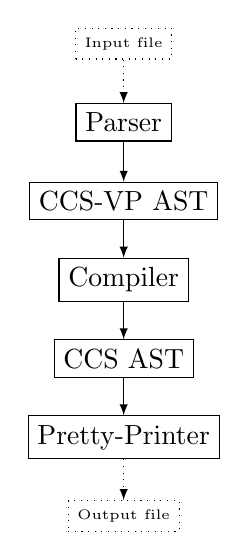
\begin{tikzpicture}[node distance=1cm, auto]
      \node (Input) [draw, dotted, rectangle] {\tiny Input file};
      \node (Parser) [draw, rectangle, align=center, below of=Input] {Parser};
      \node (VccsAST) [draw, rectangle, below of=Parser] {CCS-VP AST};
      \node (Compiler) [draw, rectangle, below of=VccsAST] {Compiler};
      \node (PccsAST) [draw, rectangle, below of=Compiler] {CCS AST};
      \node (Printer) [draw, rectangle, below of=PccsAST] {Pretty-Printer};
      \node (Output) [draw, dotted, rectangle, below of=Printer] {\tiny Output file};

      \draw [dotted, -latex] (Input) -- (Parser);
      \draw [-latex] (Parser) -- (VccsAST);
      \draw [-latex] (VccsAST) -- (Compiler);
      \draw [-latex] (Compiler) -- (PccsAST);
      \draw [-latex] (PccsAST) -- (Printer);
      \draw [dotted, -latex] (Printer) -- (Output);
    \end{tikzpicture}

    \column{0.7\textwidth}
    \begin{itemize}
      \item Implements the encoding $\enc{\cdot} : \text{CCS-VP} \to \text{CCS}$ from lecture
      \item Input: value-passing CCS with \textbf{interval-typed} parameters
      \item Parser: built with FsYacc/FsLex
      \item Compiler: structural recursion on the CCS-VP AST
      \item Output: grounded Pure CCS
    \end{itemize}

  \end{columns}

\end{frame}

% ------------------------------------------------------------------------------
% ------------------------------------------------------------------------------
% ------------------------------------------------------------------------------

\begin{frame}[fragile,c]
  \frametitle{Input Language}

  \begin{columns}[c]
    \column{0.6\textwidth}
    \begin{lstlisting}[basicstyle=\ttfamily\scriptsize]
Declaration:
P = proc;
Q(x:[L,H], y:[L,H]) = proc;

Process constructors:
'a(e).P             output
a(x:[L,H]).P        input
tau.P               silent action
P + Q               choice
P | Q               parallel
P \ {a:[L,H]}       restriction
P [a/b:[L,H]]       renaming (a to b)
if b then P else Q  conditional
K(e1,...,en)        constant call
nil                 nil
    \end{lstlisting}

    \column{0.3\textwidth}
    \textbf{Example}
    \begin{lstlisting}[basicstyle=\ttfamily\Tiny]
B  = in(x:[0,1]).'out(x).B;
B' = 'in(0).B';

Q(x:[0,2]) =
  if x != 0 then tau.Q(x-1)
  else 'done(0).nil;
    \end{lstlisting}
    \textbf{Result}
    \begin{lstlisting}[basicstyle=\ttfamily\Tiny]
B = in_0.'out_0.B + in_1.'out_1.B
B' = 'in_0.B'

Q_0 = 'done_0.0  // 0 = nil
Q_1 = tau.Q_0
Q_2 = tau.Q_1
    \end{lstlisting}
  \end{columns}

\end{frame}

% ------------------------------------------------------------------------------
% ------------------------------------------------------------------------------
% ------------------------------------------------------------------------------

\begin{frame}[c]
  \frametitle{Encoding Rules}
  \centering
  
  \tiny
  \begin{tabular}{rcl}
    $\enc{a(x{:}[L,H]).\,P}$
    & $=$ & $ \displaystyle\sum_{m=L}^{H}\; a_m \,.\, \enc{P\{^m/_x\}}$ \\[8pt]
    $\enc{\overline{a}(e).\,P}$
    & $=$ & $ \overline{a}_m \,.\, \enc{P}$ \quad ($e \!\downarrow\! m$) \\[4pt]
    $\enc{\tau.\,P}$
    & $=$ & $ \tau \,.\, \enc{P}$ \\[4pt]
    $\enc{P + Q}$
    & $=$ & $ \enc{P} + \enc{Q}$ \\[4pt]
    $\enc{P \mid Q}$
    & $=$ & $ \enc{P} \mid \enc{Q}$ \\[4pt]
    $\enc{\mathbf{0}}$
    & $=$ & $ \mathbf{0}$ \\[4pt]
    $\enc{P \setminus \{c{:}[L,H]\}}$
    & $=$ & $ \enc{P} \setminus \{\,c_L,\; c_{L+1},\; \ldots,\; c_H\,\}$ \\[4pt]
    $\enc{P\;[\,a / b {:} [L,H]\,]}$
    & $=$ & $ \enc{P}[f']$ \quad $f'(a_m)=b_m,\;\; f'(\overline{a}_m)=\overline{b}_m \quad m \in [L,H]$ \\[4pt]
    $\enc{\text{if } b \text{ then } P \text{ else } Q}$
    & $=$ & $ \begin{cases} \enc{P} & b \text{ true} \\ \enc{Q} & b \text{ false}\end{cases}$ \\[8pt]
    $\enc{K(e_1,\ldots,e_h)}$
    & $=$ & $ K_{n_1,\ldots,n_h}$ \quad ($e_i \!\downarrow\! n_i$) \\[4pt]
  \end{tabular}
  
  \vspace{0.3cm}
  
  \tiny $K_{n_1,\ldots,n_h} \;\overset{\text{def}}{=}\; \enc{P\{^{n_1}/_{x_1},\ldots,^{n_h}/_{x_h}\}}$
  \quad where $K(x_1{:}[L_1,H_1],\ldots,x_h{:}[L_h,H_h]) \overset{\text{def}}{=} P$ and $n_i \in [L_i, H_i]$
  
  \vspace{0.6cm}

  \small\textit{Each variable domain is restricted to a finite interval $[L,H]$,
  turning $\sum_{m \in \mathbb{N}}$ of the input rule into $\sum_{m=L}^{H}$.}
  
  \vspace{.2cm}
  
  \small\textit{ Restriction and Renaming rules are also adapted with channel typing.}
  
\end{frame}
  
% ------------------------------------------------------------------------------
% ------------------------------------------------------------------------------
% ------------------------------------------------------------------------------

\begin{frame}[fragile,c]
  \frametitle{Types}

  \begin{columns}[c]
    \column{0.5\textwidth}
    \centering
    \textbf{CCS-VP} \quad \texttt{(Vccs.P)}
    \begin{lstlisting}[basicstyle=\ttfamily\Tiny]
open Interval

type Action =
  | Input of string * (string * Interval) 
  | Output of string * AExp
  | Silent

type P =
  | ConstCall of string * AExp list 
  | Act of Action * P
  | Sum of P * P
  | Parallel of P * P
  | Restrict of P * (string * Interval) list
  | Rename of P * (string * string * Interval) list
  | Nil
  | Conditional of BExp * P * P

type Vccs = string * (string * Interval) list * P
    \end{lstlisting}

    \column{0.5\textwidth}
    \centering
    \textbf{CCS} \quad \texttt{(Pccs.P)}
    \begin{lstlisting}[basicstyle=\ttfamily\Tiny]
type channel = string

type Action =
  | Input of string
  | Output of string
  | Silent

type P =
  | ConstCall of string                
  | Act of Action * P                
  | Sum of P * P                   
  | Parallel of P * P               
  | Restrict of P * string list       
  | Rename of P * (Action * Action) list  
  | Nil


type Pccs = string * P
    \end{lstlisting}
  \end{columns}

  \vspace{1cm}
  \small
  \centering
  \texttt{Vccs} also contains standard declaration for arithmetic and boolean expressions, 
  that disappear, alongside \texttt{Conditional}, during compilation.

\end{frame}

% ------------------------------------------------------------------------------
% ------------------------------------------------------------------------------
% ------------------------------------------------------------------------------

\begin{frame}[c, fragile]
  \frametitle{\texttt{compile} function}

  \begin{columns}[c]

    \column{0.40\textwidth}
    \centering
    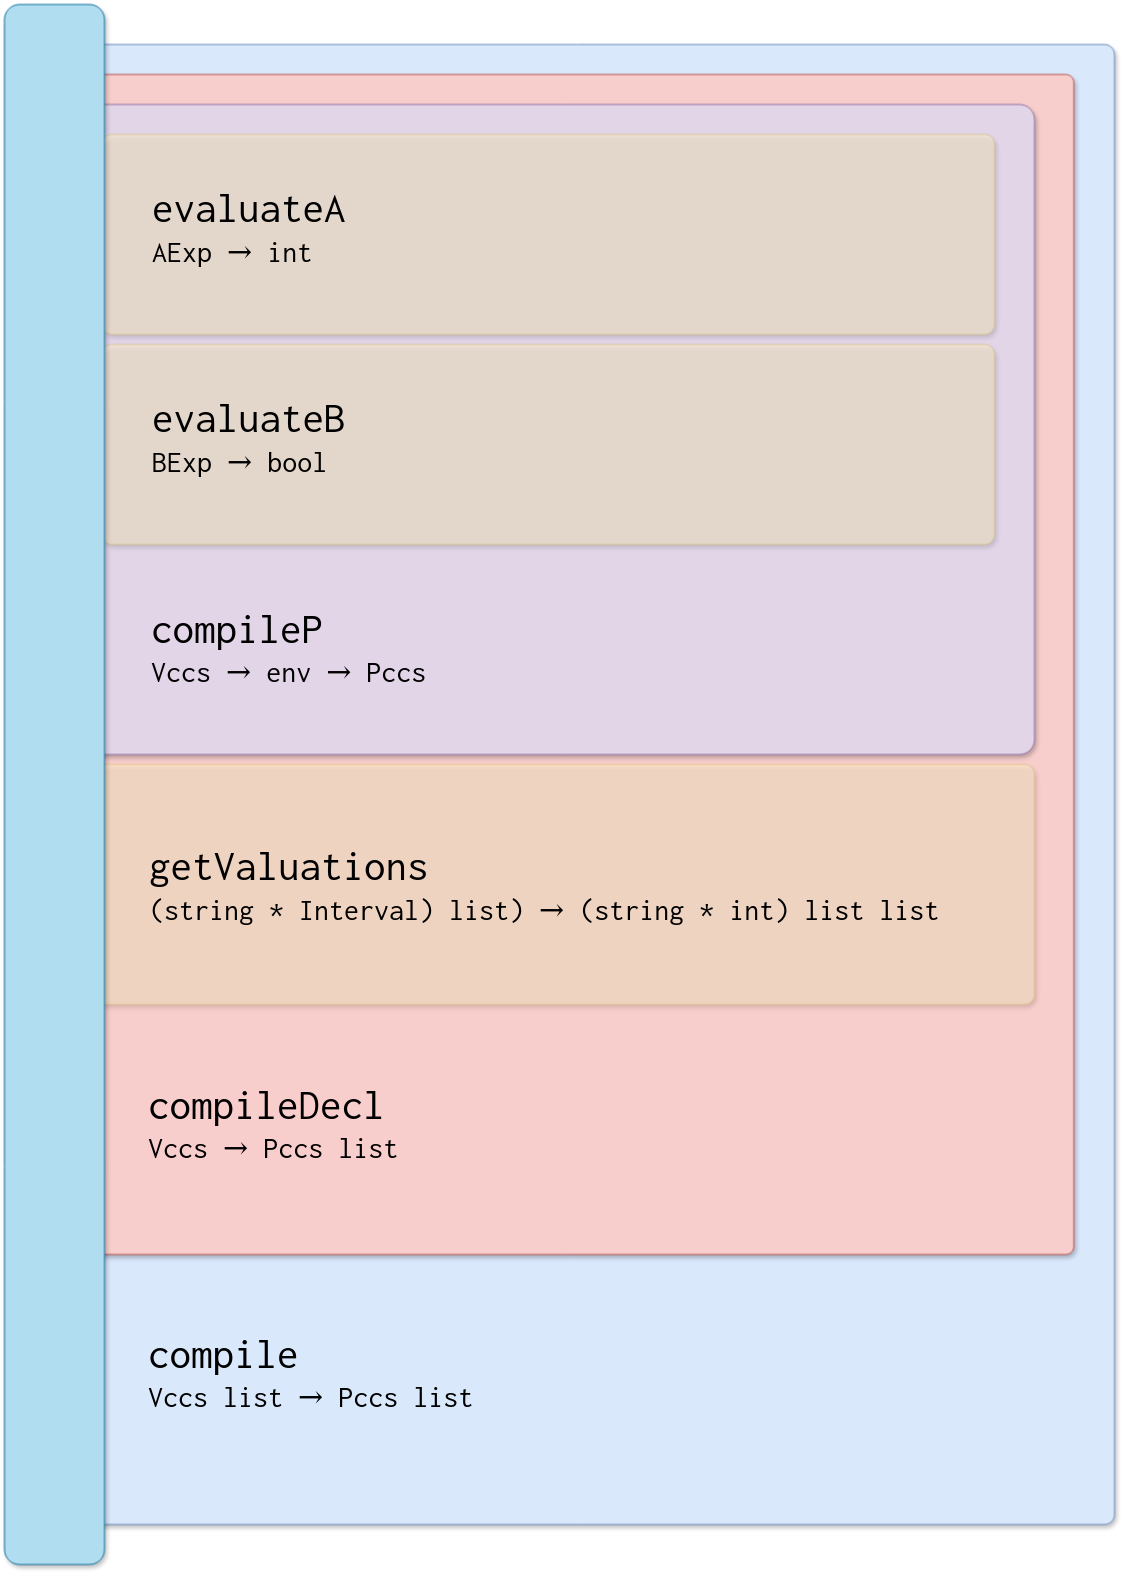
\includegraphics[width=\linewidth]{compile-function-structure.png}

    \column{0.70\textwidth}
    \begin{lstlisting}[basicstyle=\ttfamily\tiny]
let compile (vccs_list: Vccs list) : Pccs list =

  let rec compileDecl (vccs_proc: Vccs) : Pccs list =
    
    let rec compileP (Vccs -> env -> Pccs) =  
      let evaluateA = ...
      let evaluateB = ...
      :
      // Core-function

    match vccs_proc with
    | name, [], body ->
        [Pccs(name, compileP body [])]
    | name, params, body ->
        getValuations params
        |> List.map (
          fun env -> 
            Pccs(name + sfx env,compileP body env)
          )

  vccs_list |> List.collect compileDecl
    \end{lstlisting}

  \end{columns}
\end{frame}

% ------------------------------------------------------------------------------
% ------------------------------------------------------------------------------
% ------------------------------------------------------------------------------

\begin{frame}[c,fragile]
  \frametitle{\texttt{getValuations} function}
  \begin{lstlisting}[basicstyle=\ttfamily\tiny]
let getValuations (parameters: (string * Interval) list) : (string * int) list list =
  let domains = parameters |> List.map (fun (name, (lo, hi)) -> name, [lo .. hi])
  let rec cartesianProduct domains =
    match domains with
    | [] -> [ [] ]
    | (name, values) :: rest ->
      [ for value in values do
          for combo in cartesianProduct rest ->
            (name, value) :: combo ]
  cartesianProduct domains
  \end{lstlisting}

  \vspace{.5cm}

  \begin{itemize}
    \item Computes the Cartesian product of all parameter domains
    \item \textbf{Example:} \texttt{K(x:[0,1], y:[0,2])} $\mapsto$ \texttt{K\_0\_0} \ldots \texttt{K\_1\_2}
    \item \texttt{compileP body env} called once per valuation; the valuation seeds the initial \texttt{env}
  \end{itemize}

\end{frame}

% ------------------------------------------------------------------------------
% ------------------------------------------------------------------------------
% ------------------------------------------------------------------------------

\begin{frame}
  \frametitle{\texttt{compileP} function}
  \footnotesize
  \vspace{0.2cm}
  \begin{description}
    \item[\textbf{Input}] {\scriptsize\texttt{Act(Input(ch,(x,[L,H])),P)}}\\[-2pt]
                          Each $m \in [L,H]$ produces one branch compiled appending
                          $(x \mapsto m)$ to \texttt{env}, after folded into a sum
                          via \texttt{List.reduce}.
    \item[\textbf{Conditional}] {\scriptsize\texttt{Conditional(BExp,P,Q)}}\\[-2pt]
                                Guard evaluated using \texttt{evaluateB} and used to
                                tail call branch accordingly.
    \item[\textbf{Rename}] {\scriptsize\texttt{Rename(P,(from,to,[L,H]) list)}}\\[-2pt]
                           Each \texttt{(fromCh, toCh, [L,H])} generates \emph{two}
                           pairs per $m$: $(a_m \to b_m)$ and
                           $(\overline{a}_m \to \overline{b}_m)$, directly
                           implementing $f'$.
    \item[\textbf{Restrict}] {\scriptsize\texttt{Restrict(P,(ch,[L,H]) list)}}\\[-2pt]
                             Each \texttt{(ch, [L,H])} expands to
                             $\{\texttt{ch\_L},\ldots,\texttt{ch\_H}\}$ via
                             \texttt{List.collect}; the compiled process is
                             restricted to the resulting flat name list.
    \item[\textbf{ConstCall}] {\scriptsize\texttt{ConstCall(K, AExp list)}}\\[-2pt]
                              \begin{itemize}
                                \item No-argument case: name unchanged.
                                \item General case: each argument evaluated and concatenated
                                      as a suffix (\texttt{K\_1\_2}).
                              \end{itemize}
  \end{description}

  \vspace{0.2cm}
  \small\textit{Sum, Parallel, Nil, Silent, Output: structural pass-throughs.}

\end{frame}

% ------------------------------------------------------------------------------
% ------------------------------------------------------------------------------
% ------------------------------------------------------------------------------

\begin{frame}[fragile]
  \frametitle{Program}

  Two execution modes:

  \vspace{0.3cm}

  \textbf{File mode}
  \begin{lstlisting}[language={}, basicstyle=\ttfamily\tiny]
../project-root $ dotnet run input.vccs input.vccs
Parsed successfully.
Compiled successfully.
Output written to: input.ccs
  \end{lstlisting}

  \vspace{0.3cm}

  \textbf{Interactive REPL}
  \begin{lstlisting}[language={}, basicstyle=\ttfamily\tiny]
../project-root $ dotnet run 
vccs> B = in(x:[0,1]).'out(x).B;
B = (in_0.'out_0.B + in_1.'out_1.B)
vccs> B = in(x:[0,1]).'out(x).B;
B = (in_0.'out_0.B + in_1.'out_1.B)
vccs> #list
B
vccs> #clear
Context cleared.
vccs> #quit
  \end{lstlisting}

  \vspace{0.2cm}
  \small With undefined-reference warnings. And \texttt{--caal} compatible output format.

\end{frame}

% ------------------------------------------------------------------------------
% ------------------------------------------------------------------------------
% ------------------------------------------------------------------------------

\begin{frame}[fragile]
  \frametitle{Examples}

  \begin{lstlisting}[language={}, basicstyle=\ttfamily\tiny]
// Lecture Examples - Value-Passing CCS Test Suite

// --- Single-slot cell --------------------------------------------
Cell = in(x:[0,3]).CellFull(x);
CellFull(x:[0,3]) = 'out(x).Cell;

// --- Simple buffer -----------------------------------------------
Buf = recv(x:[0,3]).BufFull(x);
BufFull(x:[0,3]) = 'send(x).Buf;

// --- 2-place FIFO buffer -----------------------------------------
Fifo2 = in(x:[0,2]).Fifo1(x);
Fifo1(x:[0,2]) = 'out(x).Fifo2 + in(y:[0,2]).Fifo0(x,y);
Fifo0(x:[0,2], y:[0,2]) = 'out(x).Fifo1(y);

// --- 2-place unordered buffer ------------------------------------
Ubuf2 = in(x:[0,2]).Ubuf1(x);
Ubuf1(x:[0,2]) = 'out(x).Ubuf2 + in(y:[0,2]).Ubuf0(x,y);
Ubuf0(x:[0,2], y:[0,2]) = 'out(x).Ubuf1(y) + 'out(y).Ubuf1(x);

// --- Bounded counter ---------------------------------------------
Counter(x:[0,3]) =
  'read(x).Counter(x)
  + (if x < 3 then 'inc(x).Counter(x+1))
  + (if x > 0 then 'dec(x).Counter(x-1));

// --- Binary semaphore --------------------------------------------
Sem(s:[0,1]) =
  (if s == 0 then acquire(a:[1,1]).Sem(1))
  + (if s == 1 then release(r:[1,1]).Sem(0));

// --- Coffee machine ----------------------------------------------
CM = coin(c:[1,1]).'coffee(1).CM;
// Variant: non-deterministic choice between coffee and tea.
CMT = coin(c:[1,1]).('coffee(1).CMT + 'tea(1).CMT);

// --- Vending machine with renaming -------------------------------
VM = coin(c:[1,1]).'item(1).VM;
ChocVM = VM [item/choc:[1,1]];
TeaVM  = VM [item/tea:[1,1]];

// --- Reliable channel over lossy medium --------------------------
Sender = inp(x:[0,2]).Sending(x);
Sending(x:[0,2]) = 'medium(x).Waiting(x);
Waiting(x:[0,2]) =
  error(e:[1,1]).Sending(x) + ack(a:[1,1]).Sender;

Receiver = medium(x:[0,2]).'out(x).'ack(1).Receiver;

// --- Composed reliable channel -----------------------------------
ReliableChannel = (Sender | Receiver) \ {medium:[0,2]};

  \end{lstlisting}

\end{frame}

% ------------------------------------------------------------------------------
% ------------------------------------------------------------------------------
% ------------------------------------------------------------------------------

\begin{frame}[fragile]
  \frametitle{Results}

  \begin{lstlisting}[language={}, basicstyle=\ttfamily\tiny]
Cell = (((in_0.CellFull_0 + in_1.CellFull_1) + in_2.CellFull_2) + in_3.CellFull_3);
CellFull_0 = 'out_0.Cell;
CellFull_1 = 'out_1.Cell;
CellFull_2 = 'out_2.Cell;
CellFull_3 = 'out_3.Cell;
Buf = (((recv_0.BufFull_0 + recv_1.BufFull_1) + recv_2.BufFull_2) + recv_3.BufFull_3);
BufFull_0 = 'send_0.Buf;
BufFull_1 = 'send_1.Buf;
BufFull_2 = 'send_2.Buf;
BufFull_3 = 'send_3.Buf;
Fifo2 = ((in_0.Fifo1_0 + in_1.Fifo1_1) + in_2.Fifo1_2);
Fifo1_0 = ('out_0.Fifo2 + ((in_0.Fifo0_0_0 + in_1.Fifo0_0_1) + in_2.Fifo0_0_2));
Fifo1_1 = ('out_1.Fifo2 + ((in_0.Fifo0_1_0 + in_1.Fifo0_1_1) + in_2.Fifo0_1_2));
Fifo1_2 = ('out_2.Fifo2 + ((in_0.Fifo0_2_0 + in_1.Fifo0_2_1) + in_2.Fifo0_2_2));
Fifo0_0_0 = 'out_0.Fifo1_0;
Fifo0_0_1 = 'out_0.Fifo1_1;
Fifo0_0_2 = 'out_0.Fifo1_2;
Fifo0_1_0 = 'out_1.Fifo1_0;
Fifo0_1_1 = 'out_1.Fifo1_1;
Fifo0_1_2 = 'out_1.Fifo1_2;
Fifo0_2_0 = 'out_2.Fifo1_0;
Fifo0_2_1 = 'out_2.Fifo1_1;
Fifo0_2_2 = 'out_2.Fifo1_2;
Ubuf2 = ((in_0.Ubuf1_0 + in_1.Ubuf1_1) + in_2.Ubuf1_2);
Ubuf1_0 = ('out_0.Ubuf2 + ((in_0.Ubuf0_0_0 + in_1.Ubuf0_0_1) + in_2.Ubuf0_0_2));
Ubuf1_1 = ('out_1.Ubuf2 + ((in_0.Ubuf0_1_0 + in_1.Ubuf0_1_1) + in_2.Ubuf0_1_2));
Ubuf1_2 = ('out_2.Ubuf2 + ((in_0.Ubuf0_2_0 + in_1.Ubuf0_2_1) + in_2.Ubuf0_2_2));
Ubuf0_0_0 = ('out_0.Ubuf1_0 + 'out_0.Ubuf1_0);
Ubuf0_0_1 = ('out_0.Ubuf1_1 + 'out_1.Ubuf1_0);
Ubuf0_0_2 = ('out_0.Ubuf1_2 + 'out_2.Ubuf1_0);
Ubuf0_1_0 = ('out_1.Ubuf1_0 + 'out_0.Ubuf1_1);
Ubuf0_1_1 = ('out_1.Ubuf1_1 + 'out_1.Ubuf1_1);
Ubuf0_1_2 = ('out_1.Ubuf1_2 + 'out_2.Ubuf1_1);
Ubuf0_2_0 = ('out_2.Ubuf1_0 + 'out_0.Ubuf1_2);
Ubuf0_2_1 = ('out_2.Ubuf1_1 + 'out_1.Ubuf1_2);
Ubuf0_2_2 = ('out_2.Ubuf1_2 + 'out_2.Ubuf1_2);
Counter_0 = (('read_0.Counter_0 + 'inc_0.Counter_1) + 0);
Counter_1 = (('read_1.Counter_1 + 'inc_1.Counter_2) + 'dec_1.Counter_0);
Counter_2 = (('read_2.Counter_2 + 'inc_2.Counter_3) + 'dec_2.Counter_1);
Counter_3 = (('read_3.Counter_3 + 0) + 'dec_3.Counter_2);
Sem_0 = (acquire_1.Sem_1 + 0);
Sem_1 = (0 + release_1.Sem_0);
CM = coin_1.'coffee_1.CM;
CMT = coin_1.('coffee_1.CMT + 'tea_1.CMT);
VM = coin_1.'item_1.VM;
ChocVM = VM [choc_1/item_1];
TeaVM = VM [tea_1/item_1];
Sender = ((inp_0.Sending_0 + inp_1.Sending_1) + inp_2.Sending_2);
Sending_0 = 'medium_0.Waiting_0;
Sending_1 = 'medium_1.Waiting_1;
Sending_2 = 'medium_2.Waiting_2;
Waiting_0 = (error_1.Sending_0 + ack_1.Sender);
Waiting_1 = (error_1.Sending_1 + ack_1.Sender);
Waiting_2 = (error_1.Sending_2 + ack_1.Sender);
Receiver = ((medium_0.'out_0.'ack_1.Receiver + medium_1.'out_1.'ack_1.Receiver) + medium_2.'out_2.'ack_1.Receiver);
ReliableChannel = (Sender | Receiver) \ {medium_0, medium_1, medium_2};
  \end{lstlisting}

\end{frame}

% ------------------------------------------------------------------------------
% ------------------------------------------------------------------------------
% ------------------------------------------------------------------------------

\begin{frame}
  \frametitle{Limitations}

  \begin{enumerate}

    \item \textbf{Interval types only} \\
          Enumeration types from the spec (e.g.\ $\{a, b, c\}$) are not supported.

    \vspace{0.2cm}

    \item \textbf{Domain explosion} \\
          $n$ parameters each with domain size $d$ generate $d^n$ definitions.
          No dead-code elimination or deduplication.

    \vspace{0.2cm}

    \item \textbf{No static type checking} \\
          Undefined constant references surface only as post-compilation
          warnings, not as errors before code generation.

  \end{enumerate}

\end{frame}

\end{document}
